\documentclass[8pt,landscape]{article}

% PACKAGES
\usepackage[letterpaper, margin=0.1in]{geometry}
\usepackage{amsmath, amssymb, geometry}
\usepackage{multicol}
\usepackage{setspace}
\usepackage{sectsty}
\usepackage{verbatim}
\usepackage{graphicx}
\usepackage{xcolor}
\usepackage{listings}
\usepackage{enumitem}
\usepackage{booktabs} % For better tables if needed

% Define a custom color for code highlighting and environment
\definecolor{myred}{RGB}{204, 0, 0} % A strong red
\definecolor{mygray}{RGB}{240, 240, 240} % Light gray for background
\setlist[itemize]{
    noitemsep,  % Removes vertical space between list items
    topsep=0pt,  % Removes space before the list
    partopsep=0pt, % Removes extra space when a list begins mid-paragraph
    parsep=0pt, % Removes space between paragraphs within an item
    leftmargin=*, % Sets the left margin to the minimum necessary
    labelsep=0.5em, % You can slightly adjust the space between the bullet and the text
}
% LISTINGS SETUP for R and Python
\lstset{
  basicstyle=\ttfamily\scriptsize\color{black},
  backgroundcolor=\color{mygray},
  frame=single,
  frameround=tttt,
  framesep=0pt,        % no padding between code and frame
  rulecolor=\color{black!20},
  rulesep=0pt,         % no space between rules
  breaklines=true,
  columns=fullflexible,
  showstringspaces=false,
  commentstyle=\color{gray},
  keywordstyle=\color{blue!80!black},
  stringstyle=\color{myred},
  breakatwhitespace=true,
  xleftmargin=0pt,     % no left margin
  xrightmargin=0pt,    % no right margin
  aboveskip=0pt,       % no space above listing
  belowskip=0pt,       % no space below listing
  abovecaptionskip=0pt,
  belowcaptionskip=0pt,
  framexleftmargin=0pt,
  framexrightmargin=0pt,
  framextopmargin=0pt,
  framexbottommargin=0pt
}

% FORMATTING
\setstretch{0.9} % Reduce line spacing
\setlength{\parindent}{0pt}
\setlength{\parskip}{0pt}

% Reduce section spacing and change color
\makeatletter
\renewcommand{\section}{\@startsection{section}{2}{0pt}%
    {0.1ex}% space before section
    {0.1ex}% space after section
    {\fontsize{8}{9}\bfseries\color{red}}} % section font: 8pt
\makeatother

% Reduce subsection spacing and make subsections blue
\makeatletter
\renewcommand{\subsection}{\@startsection{subsection}{2}{0pt}%
    {0.1ex}% space before subsection
    {0.1ex}% space after subsection
    {\fontsize{8}{9}\bfseries\color{blue}}} % Subsection font: 8pt
\makeatother

% Custom command for red-highlighted code/commands (for in-line use)
\newcommand{\code}[1]{\textcolor{myred}{\texttt{#1}}}

% Custom small text wrapper - ensuring 8pt for body text
\newcommand{\smalltext}[1]{
  {\fontsize{8}{9}\selectfont\sloppy #1\par}
}

% DOCUMENT START
\begin{document}
\fontsize{8}{9}\selectfont % Set the base font size to 8pt and line skip to 9pt for the entire document
\pagestyle{empty}
\begin{multicols}{3}


% \section{Features of a TS}
% \smalltext{
%   Univariate: A TS that consists of a single variable recorded sequentially over time (e.g., bike sale over time from a single store)
%   Multivariate: Consists of multiple variables recorded sequentially over time (e.g., bike sale and profit over time from a single store)
%   Hierachical: Consists of multiple variables from multiple observations, nested within the larger group categories, recorded sequentially over time (e.g., bike sale and profit from multiple stores over time)
% }

\section{Working with TS - Temporal dependence}
\smalltext{
  \textbf{Correlogram} Plots the autocorrelation function (ACF). If ACF for residuals diagnostics as part of the ARIMA routine, the standard errors are determined assuming the residuals are white noise.
If ACF used as part of the raw data as a model selection tool, then we should use the Bartlett's formula. `bartlett\_confint=True`
}
\begin{lstlisting}[language=python]
  plot_acf(sun["sunspots"], lags=50, title="ACF of Sunspots")
\end{lstlisting}

\subsection{Time Series (TS) Patterns}
\smalltext{
  \textbf{Trend:} long term increases or decreases in the series. Patterns that don't repeat with a regular period.

  \textbf{Seasonality:} regular variation in the series at some fixed interval, e.g., month, day of week, time of day, etc.

  \textbf{Cyclicity:} variations in the series that repeat with some regularity but of unknown and changing period.

  Seasonal smaller timeframe than cyclical, but at a fixed frequency.
  Cyclical larger timeframe than seasons, and not at a fixed frequency.
  Cyclical always larger timeframe than seasonal behaviour.

  \textbf{White noise:} Zero mean, constant variance, no autocorrelation, iid and Gaussian.
  It means the TS of random numbers and cannot be predicted.
  Residuals/errors from a TS for a forecast model should resemble white noise, implies that we have extracted all the useful information from the TS.
}

\section{Time series decomposition}
\smalltext{
\textbf{Additive}
Appropriate if the magnitude of the seasonal fluctuations, or the variation around the trend-cycle, does not vary with the value of the series.
\textbf{Multiplicative}
Appropriate if variation in the seasonal pattern, or the variation around the trend-cycle, appears to be proportional to the value of series.
}
\smalltext{
\textbf{When to use which:} Look at the \textbf{size of seasonal swings} (and variation around the trend) over time.
  \textbf{Additive} if that size is roughly \textbf{constant} (same ± swing at low and high levels). \textbf{Multiplicative} if swings/variation \textbf{grow with the level} (e.g., higher trend $\Rightarrow$ bigger seasonal amplitude or spread). Series that grow a lot or span a wide range often need multiplicative; stable-range series often additive.
}

\textbf{Estimating the trend-cycle (T)}
\textbf{Curve-fitting}
\smalltext{
  Easily calculate and remove a simple polynomial curve from our data.
}

\textbf{Moving average}
\smalltext{
  Passing a window of some size over the data and calculating the average.
  Nature of data, expert knowledge, tells window size. If seasonality in the data, use a window equal to the seasonal period. 
 Period other than 12 may contaminate the trend-cycle with seasonality.
  \textbf{Problem with MA of even window size} moving average doesn't line up with the index of the original series. To rectify this, we usually take an extra 2-MA of the result of a MA with an even window.
}

\textbf{Estimating the Seasonality (S)}
\smalltext{
1. Remove the trend-cycle component from the data
2. Estimate the seasonal component by averaging
}

\textbf{Estimating the remainder (R)}
\smalltext{
  Simply subtract the trend-cycle and seasonal components from the original series.
}

\begin{lstlisting}[language=python]
#Use seasonal_decompose or STL
model = seasonal_decompose(co2[["CO2"]],model="additive",period=12)
model = STL(co2["CO2"], period=12, seasonal=13).fit() #STL 
\end{lstlisting}

\section{Forecasting}
\smalltext{
  \textbf{Average} Use the average of the series for all future forecasts.

  \textbf{Naive} Use the last observation for all forecasts.

  \textbf{Seasonally-adjusted Naive} seasonally adjusted by applying a classical decomposition.

  \textbf{Seasonal Naive} Set each forecast as the last observed value from the same season of the year.

  \textbf{Drift} Forecasts equal to last value in the series plus the average change of the series.
  $\hat{y}_{T+h|T} = y_T + h \left( \frac{y_T - y_1}{T - 1} \right)$
}

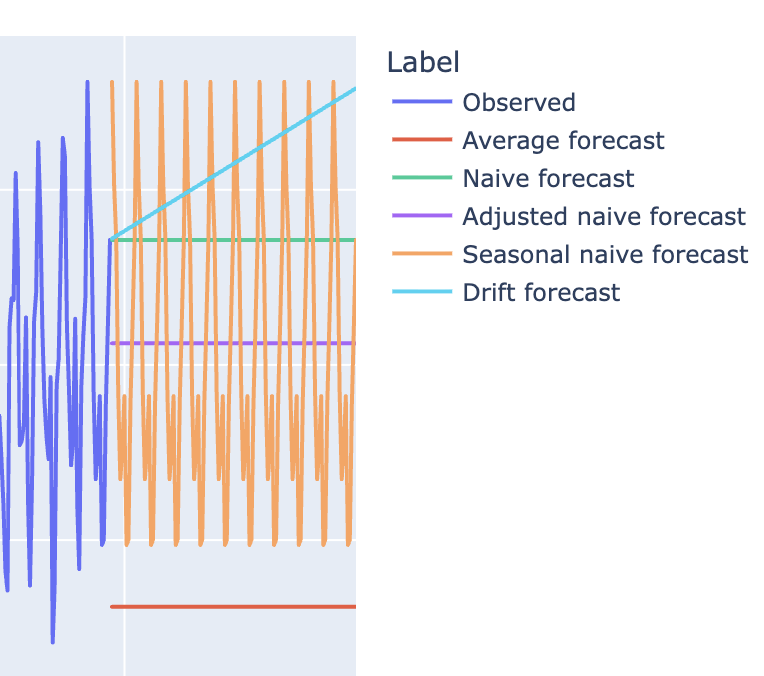
\includegraphics[width=0.3\linewidth, height=2cm]{forecasting.png}
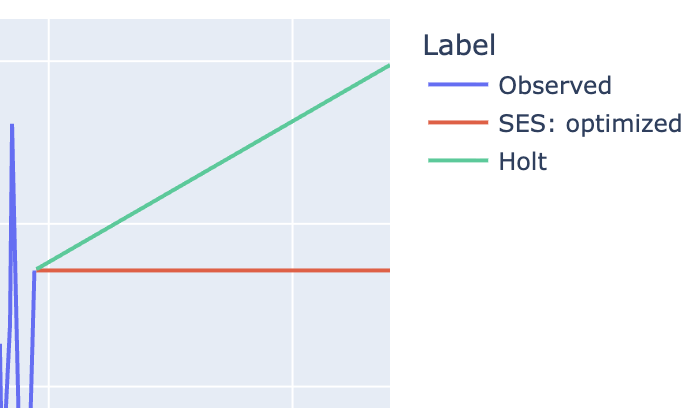
\includegraphics[width=0.3\linewidth, height=2cm]{holt.png}
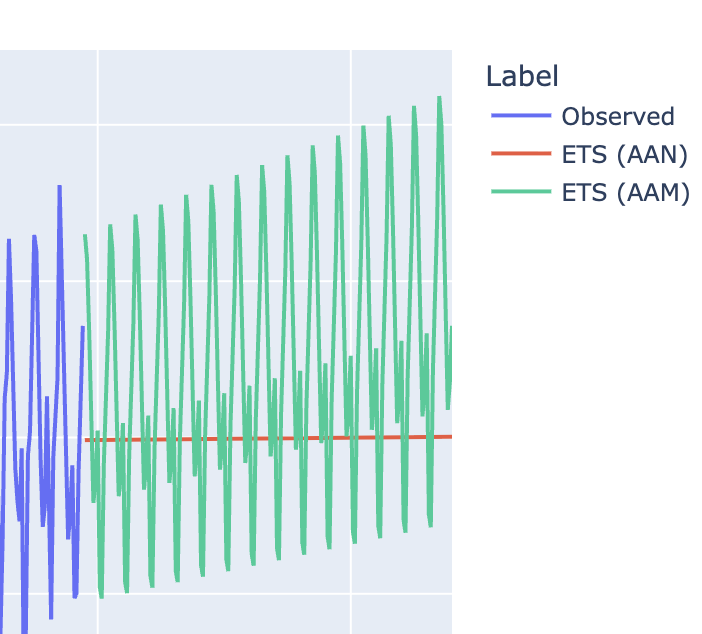
\includegraphics[width=0.3\linewidth, height=2cm]{ETS.png}

\subsection{Simple Exponential Smoothing (SES)}
\smalltext{
  \textbf{Focus:} Level only. Best for data with no clear trend or seasonality.
  \textbf{$\alpha$ (Smoothing):} Controls the "memory." 
  \textbf{High $\alpha \to 1$:} Short-term memory (reacts quickly to the very last observation).
  \textbf{Low $\alpha \to 0$:} Long-term memory (stable, uses a long history of data).
}

\textbf{Holt's Method (Trend)}
\smalltext{
  \textbf{Focus:} Level + Trend. Use when data has a consistent direction.
  \textbf{$\beta$ (Trend):} Controls how fast the slope changes.
  \textbf{High $\beta \to 1$:} Trend updates rapidly (changes with every new point).
  \textbf{Low $\beta \to 0$:} Trend is more linear/constant over time.
}

\textbf{Holt-Winter's Method (Seasonality)}
\smalltext{
  \textbf{Focus:} Level + Trend + Seasonality. Best for data with repeating patterns.
  \textbf{$\gamma$ (Seasonality):} Controls seasonal flexibility.
  \textbf{High $\gamma \to 1$:} Seasonal pattern updates fast (Seasonal Naive).
  \textbf{Low $\gamma \to 0$:} Seasonal pattern stays fixed (Global Average).
}

\textbf{Key Takeaways:}
    \textbf{Parameter Logic:} All parameters ($\alpha, \beta, \gamma$) range from 0 to 1. Higher = More reactive; Lower = More stable.
    \textbf{Optimization:} We typically choose these values by minimizing \textbf{SSE} (Sum of Squared Errors).
    \textbf{Versatility:} There are 9 possible combinations of Trend (None, Additive, Multiplicative) and Seasonality.

\textbf{ETS method}
\smalltext{
  If we want to also generate prediction intervals.
  ETS models optimize by maximizing the likelihood.
}


\section{Model selection}

\smalltext{  
  \textbf{AIC, BIC - Lowest better,}
  \textbf{Visual inspection} (residuals should be uncorrelated, have zero mean, and ideally be normally distributed)
  Ljung-Box	Autocorrelation	High p-value (Residuals are white noise; no remaining patterns.)
  Jarque-Bera	Normality	High p-value (Residuals are approximately normal.)
  \textbf{Out-of-sample methods} (MAE) (RMSE) (MAPE) (MASE) MAE and RMSE are popular in practice because they are easier to interpret. Closer to 0 is better. MAPE is scale-free and aims to proportionalize errors.MAPE is problematic if 0 values are expected (divide by 0 error) and it is also not symmetrical. MASE scales the MAE based on the MAE of a naive forecast on the training data. 
}

\section{Stationary}
\smalltext{
  A constant mean and variance. No strong up or down trends. Does not show predictable patterns (e.g., seasonality)
  \textbf{Strong stationarity,} also called strict stationarity, all moments of the time series, including its joint distribution, remain constant over time.
  \textbf{Weak stationarity, }also called second-order stationarity, is a less strict form of stationarity than strong stationarity. A time series is considered weakly stationary if its mean, variance, and autocovariance are constant over time, but its higher-order moments (such as skewness and kurtosis) may not be constant. 
}
\subsection{Check stationary}
\smalltext{
  \textbf{Visual inspections} Line plot-noticeable trend, seasonality, or changing variance over time. Correlogram-ACF plot should decay rapidly to 0. Non-stationary time-series will have ACF decays slowly.

  \textbf{Summary statistics} For stationary time series, the mean and variance should be approximately constant over time.

  \textbf{Hypothesis tests} Augmented Dickey Fuller (“ADF”) test or Kwiatkowski-Phillips-Schmidt-Shin (“KPSS”) test: Null hypo $H_0$: The time series is non-stationary, small p-value indicates stationary.   result = adfuller(noise)
}
\textbf{How to make stationary?}
\smalltext{
  \textbf{Stabilize the variance:} Log transformation is easy to interpret. Box-Cox transformation using the scipy.stats.boxcox function.
  \textbf{Stabilize the mean:} calculate the differences between consecutive observations in the series. This removes any trend in the data, since it measures the change between two points in time rather than the absolute value. 
  In some situations, 1st order data will not appear to be stationary, 2nd order to obtain a stationary series.
  If still appear non-stationarity, then you might want to check for seasonal differencing.
}
\section{Autoregressive (AR) Moving average (MA)}
\smalltext{
  We can combine autoregression + moving average, to get the dynamics of both models.
}
\smalltext{
  \textbf{AR - Long memory} every current value is built directly upon the previous value, creating a "chain reaction" that carries information from the distant past into the present.
  \textbf{Concept:} Forecasts based on \textbf{past values} ($y_{t-1}, y_{t-2}$).
  \textbf{Strength:} Captures long-term trends and persistent patterns (e.g., economic cycles).
  \textbf{Memory:} Long/Persistent. The influence of a past value decays slowly over time.
  \textbf{Weakness:} Less effective at filtering out short-term noise or random "shocks."
}
\smalltext{
  \textbf{MA - Short memory} they are built using a "sliding window" of past errors (shocks). In a standard $MA(q)$ model, the value $y_t$ is determined by the current error term and the $q$ previous error terms. correlation is non-zero for $q$ periods and then drops to exactly zero.
  Moving average model uses past forecast errors in a regression-like model.
  \textbf{Concept:} Forecasts based on \textbf{past errors} (shocks/noise). 
  \textbf{Strength:} Excellent at absorbing sudden, temporary spikes. Allows a "shock" to propagate for a fixed time.
  \textbf{Memory:} Short/Finite. Correlation is non-zero for $q$ periods, then drops to \textbf{exactly zero}.
  \textbf{Weakness:} Cannot distinguish between a temporary fluctuation and a permanent change in trend.
}


\textbf{ARIMA(p,d,q)}
\smalltext{(Autoregressive Integrated Moving Average) is just an ARMA model with differencing built-in!
p is the autoregressive order,
d is the order of differencing to apply (usually 1),
q is the moving average order
}
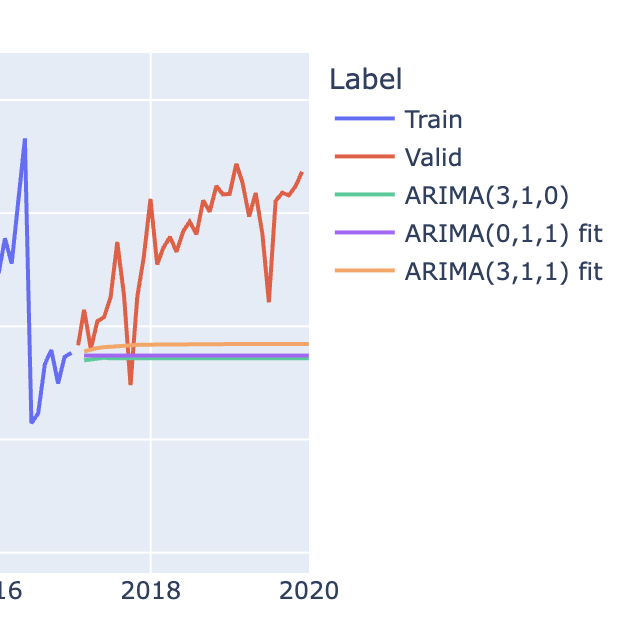
\includegraphics[width=0.5\linewidth, height=2cm]{ARIMA.png}
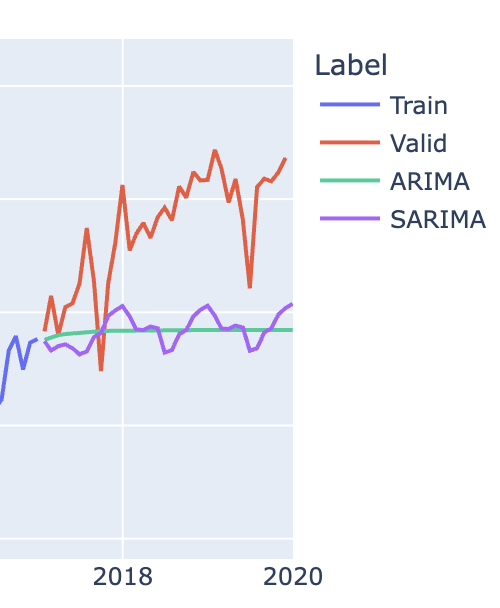
\includegraphics[width=0.5\linewidth, height=2cm]{SARIMA.png}

\smalltext{
 \textbf{SARIMA} simply adds an ARIMA with seasonal terms, that is, seasonal difference, and seasonally-based AR and MA models. It is often denoted ARIMA(p,d,q)(P,D,Q,m), where m is the seasonal period.

 \textbf{Auto-arima} The function performs a search (either stepwise or parallelized) over possible model and seasonal orders within the constraints provided, and selects the parameters that minimize the given metric.
}

\subsection{Using correlograms ACF/PACF for Choosing Order}
\smalltext{
  For an AR($p$) process: The PACF. If the PACF has significant spikes at lag 1 and 2, but then drops into the "noise zone" (insignificance) at lag 3, you likely have an AR(2) model.
  The ACF will decay slowly because of that "long-term memory".
  \textbf{Definition} Measures the direct correlation between $y_t$ and $y_{t-k}$ after removing the effects of all shorter lags (the "middle" values).What it captures: It isolates the "pure" relationship between the current value and a specific past value.

  For an MA($q$) process: The ACF. If the ACF spikes at lag 1 and then immediately hits zero, you have an MA(1).
  The PACF will decay gradually as the model's short-term shocks.
  \textbf{Definition:} Measures the total correlation between a time series and a lagged version of itself (e.g., $y_t$ and $y_{t-k}$).What it captures: It includes both direct correlation and indirect correlation (the influence of intervening time steps)
}


\subsection*{Data Splitting \& Validation}
\begin{itemize}[leftmargin=*]
    \item \textbf{Temporal Ordering:} Never shuffle data. Future data points cannot be used to predict the past (prevents data leakage).
    \item \textbf{Sliding Window CV:} A fixed-length training window "slides" forward through time. Useful if older data becomes irrelevant.
    \item \textbf{Expanding Window CV:} The training set starts small and grows as it incorporates more historical data at each fold.
\end{itemize}

\subsection*{Feature Engineering (Tabularization)}
\begin{itemize}[leftmargin=*]
    \item \textbf{Reduction:} Converting a time series forecasting problem into a standard supervised learning (regression) problem.
    \item \textbf{Lagged Features:} Using past observations ($y_{t-1}, y_{t-2}, \dots$) as input features for $X$.
    \item \textbf{Window Length ($w$):} The number of past lags used to predict the next value.
    \item \textbf{Rolling Statistics:} Features derived from a window of time, such as rolling means, standard deviations, or max/min.
\end{itemize}

\subsection*{Multi-Step Forecasting Strategies}
\begin{itemize}[leftmargin=*]
    \item \textbf{Recursive (Iterative):} Predicts $t+1$, then uses that prediction as an input to predict $t+2$. 
        \begin{itemize}
            \item \textit{Pros:} Simple, one model needed. \textit{Cons:} Error accumulation/propagation.
        \end{itemize}
    \item \textbf{Direct:} Trains a separate, independent model for each step in the horizon (e.g., Model 1 for $t+1$, Model 2 for $t+2$).
        \begin{itemize}
            \item \textit{Pros:} No error propagation. \textit{Cons:} High computational cost; ignores dependencies between steps.
        \end{itemize}
    \item \textbf{Multi-output:} A single model that produces a vector of predictions for the entire horizon at once (e.g., certain Neural Networks).
\end{itemize}

\end{multicols}
\end{document}
